\documentclass[12pt]{article}
\usepackage[left=1cm, right=1cm, top=2cm,bottom=1.5cm]{geometry} 

\usepackage[parfill]{parskip}
\usepackage[utf8]{inputenc}
\usepackage[T2A]{fontenc}
\usepackage[russian]{babel}
\usepackage{enumitem}
\usepackage[normalem]{ulem}
\usepackage{amsfonts, amsmath, amsthm, amssymb, mathtools}
\usepackage{tabularx}
\usepackage{hhline}

\usepackage{accents}
\usepackage{fancyhdr}
\pagestyle{fancy}
\renewcommand{\headrulewidth}{1.5pt}
\renewcommand{\footrulewidth}{1pt}

\usepackage{graphicx}
\usepackage[figurename=Рис.]{caption}
\usepackage{subcaption}
\usepackage{float}

%%Наименование папки откуда забирать изображения
\graphicspath{ {./images/} }

%%Изменение формата для ввода доказательства
\renewcommand{\proofname}{$\square$  \nopunct}
\renewcommand\qedsymbol{$\blacksquare$}

%%Изменение отступа на таблицах
\addto\captionsrussian{%
	\renewcommand{\proofname}{$\square$ \nopunct}%
}
%% Римские цифры
\newcommand{\RN}[1]{%
	\textup{\uppercase\expandafter{\romannumeral#1}}%
}

%% Для удобства записи
\newcommand{\MR}{\mathbb{R}}
\newcommand{\MQ}{\mathbb{Q}}
\newcommand{\MN}{\mathbb{N}}
\newcommand{\MI}{\mathrm{I}}
\newcommand{\MJ}{\mathrm{J}}
\newcommand{\MH}{\mathrm{H}}
\newcommand{\MT}{\mathrm{T}}
\newcommand{\MU}{\mathcal{U}}
\newcommand{\MV}{\mathcal{V}}
\newcommand{\VN}{\varnothing}
\newcommand{\VE}{\varepsilon}

\theoremstyle{definition}
\newtheorem{defn}{Опр:}
\newtheorem{rem}{Rm:}
\newtheorem{prop}{Утв.}
\newtheorem{exrc}{Упр.}
\newtheorem{lemma}{Лемма}
\newtheorem{theorem}{Теорема}
\newtheorem{corollary}{Следствие}

\newenvironment{cusdefn}[1]
{\renewcommand\thedefn{#1}\defn}
{\enddefn}

\DeclareRobustCommand{\divby}{%
	\mathrel{\text{\vbox{\baselineskip.65ex\lineskiplimit0pt\hbox{.}\hbox{.}\hbox{.}}}}%
}
%Короткий минус
\DeclareMathSymbol{\SMN}{\mathbin}{AMSa}{"39}
%Длинная шапка
\newcommand{\overbar}[1]{\mkern 1.5mu\overline{\mkern-1.5mu#1\mkern-1.5mu}\mkern 1.5mu}
%Функция знака
\DeclareMathOperator{\sgn}{sgn}

%Обозначение константы
\DeclareMathOperator{\const}{\text{const}}

%Интеграл в большом формате
\DeclareMathOperator{\dint}{\displaystyle\int}

\newcommand{\smallerrel}[1]{\mathrel{\mathpalette\smallerrelaux{#1}}}
\newcommand{\smallerrelaux}[2]{\raisebox{.1ex}{\scalebox{.75}{$#1#2$}}}

\newcommand{\smallin}{\smallerrel{\in}}
\newcommand{\smallnotin}{\smallerrel{\notin}}

\newcommand*{\medcap}{\mathbin{\scalebox{1.25}{\ensuremath{\cap}}}}%
\newcommand*{\medcup}{\mathbin{\scalebox{1.25}{\ensuremath{\cup}}}}%

\makeatletter
\newcommand{\vast}{\bBigg@{3.5}}
\newcommand{\Vast}{\bBigg@{5}}
\makeatother

%Скалярное произведение
\DeclarePairedDelimiterX{\inner}[2]{\langle}{\rangle}{#1, #2}

%Подпись символов снизу
\newcommand{\ubar}[1]{\underaccent{\bar}{#1}}

\begin{document}
\lhead{Математический анализ - \RN{2}}
\chead{Шапошников С.В.}
\rhead{Лекция - 18}
\section*{Дифференциалы высоких порядков}
\subsection*{Дифференциалы $m$-го порядка}
\begin{defn}
	Пусть $f\colon \MR^n \to \MR$ $m$-раз дифференцируема в точке $a$, тогда выражение:
	$$
		d^mf(a,h) = \displaystyle \sum\limits_{i_1 \dotsc i_m}\dfrac{\partial^m f}{\partial x_{i_1} \dotsc \partial x_{i_m}}(a){\cdot}h_{i_1}{\cdot}\dotsc{\cdot}h_{i_m}, \, i_j \in \{1, \dotsc, n\}, \, \forall j = \overline{1,m}
	$$
	называется \uwave{дифференциалом} $m$-\uwave{го порядка} в точке $a$ на векторе $h$.
\end{defn}
\begin{prop}
	Пусть $f\colon \MR^n \to \MR$ $m$-раз дифференцируема в точке $a$, тогда верно следующее равенство:
	$$
		d^{m}f(a,h) = d\big(d^{m-1}f(x,h)\big)(a,h)
	$$
\end{prop}
\begin{proof}
	По определению:
	$$
		d\big(\underbrace{d^{m-1}f(x,h)}_{g(x)}\big)(a,h) = \displaystyle \sum\limits_{i_m = 1}^{n}\dfrac{\partial g}{\partial x_{i_m}}(a){\cdot}h_{i_m} = \displaystyle \sum\limits_{i_m = 1}^{n}\dfrac{\partial }{\partial x_{i_m}}
		\bigg(\displaystyle \sum\limits_{i_1 \dotsc i_{m-1}}\dfrac{\partial^{m-1} f}{\partial x_{i_1} \dotsc \partial x_{i_{m-1}}}(x){\cdot}h_{i_1}{\cdot}\dotsc{\cdot}h_{i_{m-1}}\bigg)\bigg|_{x = a}{\cdot}h_{i_m} = 
	$$
	$$
		=	\displaystyle \sum\limits_{i_m = 1}^{n} \displaystyle \sum\limits_{i_1 \dotsc i_{m-1}}\dfrac{\partial^m f}{\partial x_{i_1} \dotsc \partial x_{i_m}}(a) h_{i_1}{\cdot}\dotsc{\cdot}h_{i_m} = d^m f(a,h)
	$$
\end{proof}
\begin{lemma}
	Пусть $f$ $m$-раз дифференцируема в окрестности точки $a$. Возьмем функцию $\varphi(t) = f(a + th)$. Тогда она $m$ раз дифференцируема в окрестности нуля и $m$-ая производная равна:
	$$
		\varphi^{(m)}(t) = d^mf(a + th,h)
	$$
	В частности, в нуле она равна значению $m$-го дифференциала в точке $a$ на векторе $h$: 
	$$
		\varphi^{(m)}(0) = d^mf(a,h)
	$$
\end{lemma}

\textbf{\uline{Смысл $m$-го дифференциала $\varphi(t)$}}: Пусть есть точка $a$ и есть вектор $h$, возьмем прямую натянутую на этот вектор $h$ и ограничим на неё функцию $f \Rightarrow$ функцией $f$ на этой прямой будет $\varphi(t)$.
\begin{figure}[H]
	\centering
	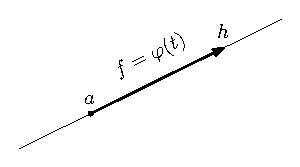
\includegraphics[width=0.25\textwidth]{18_1.eps}
	\caption{Функция $\varphi(t)$ на прямой, натянутой на вектор $h$.}
	\label{18_1}
\end{figure}
Следовательно, мы получили функцию одной переменной и если хотим понимать как она ведет себя на этой прямой, то для многих вопросов нам важно знать как устроены дифференциалы $f$. Например: 
$$
	\varphi^\prime(0) = df(a,h), \, \varphi^{\prime\prime}(0) = d^2f(a,h), \, \dotsc
$$
То есть выражая производные $\varphi$ через производные $f$ мы получаем $m$-ые дифференциалы в квадратичной форме (ещё одна причина, почему используются не полилинейные формы, а квадратичные).
\begin{proof}
	Возьмем функцию $\varphi(t) = f(a + th)$, докажем утверждение индукцей по $m$:\\
	\uline{База}: $m = 1 \Rightarrow$ продифференцируем $\varphi(t)$ как сложную функцию:
	$$
		\varphi^\prime(t) = \dfrac{\partial f}{\partial x_1}(a + th){\cdot}\dfrac{\partial x_1}{\partial t} + \dotsc + \dfrac{\partial f}{\partial x_n}(a + th){\cdot}\dfrac{\partial x_n}{\partial t} =
	$$
	$$	
	 	= \dfrac{\partial f}{\partial x_1}(a + th){\cdot}h_1 + \dotsc + \dfrac{\partial f}{\partial x_n}(a + th){\cdot}h_n = df(a + th, h)
	$$
	где последнее равенство выполняется по определению. Таким образом $\varphi^\prime(t) = df(a + th,h)$. Это также можно было найти, применив правило дифференцирования сложной функции:
	$$
		d\varphi =df \circ d(a + th) = df\big(a + th, h{\cdot}dt \big) = df\big(a + th, h \big) {\cdot}dt = \varphi^\prime(t){\cdot}dt
	$$	
	Учитывая, что $d(a+th)(t_0,v) = a + (t_0 + v){\cdot}h - a - t_0{\cdot}h = h{\cdot}v = h{\cdot}dt(t_0,v)$ мы можем записать выражение выше детальнее:
	$$
		d\varphi(t_0,v) = \big(df \circ d(a + th)\big)(t_0,v) = df\big(a + t_0h, d(a+th)(t_0,v) \big) = df\big(a + t_0h, h \big){\cdot}dt(t_0,v)
	$$
	Таким образом $d\varphi(v) = df(a + t_0h,h){\cdot}dt(v)$ и если не записываем в конкретной точке, то оно будет иметь следующий вид: 
	$$
		d\varphi = df(a + th,h){\cdot}dt = \varphi^\prime(t){\cdot}dt
	$$
	\uline{Шаг}: Предположим, что для $m$ верно, докажем для $m+1$:
	$$
		\varphi^{(m+1)}(t) = (\varphi^{(m)}(t))^\prime = \big(d^mf(a + th, h)\big)^\prime = \big(g(a +th)\big)^\prime
	$$
	где $g(x) = d^mf(x,h)$, тогда в терминах функции $g(x)$, используя случай $m=1$ и применяя предыдущее утверждение мы получим следующее:
	$$
		\big(g(a +th)\big)^\prime = dg(a + th, h) = d^{m+1}f(a + th,h)
	$$
	Таким образом, требуемое выполнено.
\end{proof}

\newpage
\section*{Формула Тейлора}
\begin{theorem}\textbf{(формула Тейлора с остаточным членом в виде Лагранжа)}
	Пусть $f$ $(m+1)$-раз дифференцируема в шаре $B(a,r)$. Тогда $\forall h \in B(0,r), \, \exists \, c \in (0,1)$ такой, что:
	$$ 
		f(a+h) = f(a) + df(a,h) + \dfrac{d^2f(a,h)}{2!} + \dotsc + \dfrac{d^mf(a,h)}{m!} + \dfrac{d^{m+1}f(a + ch,h)}{(m+1)!}
	$$
\end{theorem}
\begin{rem}
	Нужно заметить, что $c$ зависит от $h$, то есть: $c = c(h)$.
\end{rem}
\begin{proof}
	Рассмотрим функцию $\varphi(t) = f(a + th)$, она $(m+1)$-раз дифференцируема на отрезке $[0,1]$ по предыдущей лемме, поскольку по условию верно следующее: 
	$$
		\|h\| < r \Rightarrow a + th \in B(a,r), \, \forall t \in [0,1] 
	$$
	Применим формулу Тейлора для функции одной переменной $\varphi$ на отрезке $[0,1]$ и возьмем $t=1$:
	$$
		\varphi(1) = \varphi(0) + \varphi^\prime(0){\cdot}1 + \dfrac{\varphi^{\prime\prime}(0){\cdot}1^2}{2!} + \dotsc + \dfrac{\varphi^{m+1}(c)}{(m+1)!}, \, c \in (0,1)
	$$
	Подставим сюда выражение для $f$ и воспользуемся предыдущей леммой:
	$$
		f(a + h) = f(a) + df(a,h) + \dotsc + \dfrac{d^mf(a,h)}{m!} + \dfrac{d^{m+1}f(a + ch,h)}{(m+1)!}, \, c \in (0,1)
	$$
\end{proof}

\begin{theorem}\textbf{(формула Тейлора с остаточным членом в виде Пеано)}
	Пусть $f$ $m$-раз дифференцируема в окрестности точки $a$ и её производные $m$-го порядка непрерывны в точке $a$. Тогда:
	$$
		f(a+h) = f(a) + df(a,h) + \dfrac{d^2f(a,h)}{2!} + \dotsc + \dfrac{d^mf(a,h)}{m!} + \overline{o}(\|h\|^m)
	$$
\end{theorem}
\begin{rem}
	Утверждение верно без требований к непрерывности производных и без дифференцируемости в окрестности точки $a$, но без этих условий доказательство становится сложнее.
\end{rem}

\begin{proof}
	Функция $f$ $m$-раз дифференцируема в окрестности точки $a \Rightarrow$ для достаточно малых $h$ имеем следующее равенство:
	$$
		f(a + h) = f(a) + df(a,h) + \dotsc + \dfrac{d^{m-1}f(a,h)}{(m-1)!} + \dfrac{d^mf(a+ch,h)}{m!} , \, c = c(h) \in (0,1)
	$$
	Перепишем последнее слагаемое в виде:
	$$
		\dfrac{d^mf(a+ch,h)}{m!} = \dfrac{d^mf(a,h)}{m!} + \dfrac{d^mf(a+ch,h)- d^mf(a,h)}{m!} = \dfrac{d^mf(a,h)}{m!} + R
	$$
	Мы хотим проверить, что $R =\overline{o}(\|h\|^m)$. Распишем выражение $m!R$ подробнее:
	$$
		m!R = \displaystyle \sum\limits_{i_1\dotsc i_m}\bigg(\dfrac{\partial^m f(a + ch)}{\partial x_{i_1}\dotsc\partial x_{i_m}} - \dfrac{\partial^m f(a)}{\partial x_{i_1}\dotsc\partial x_{i_m}} \bigg){\cdot}h_{i_1}{\cdot}\dotsc{\cdot}h_{i_m} = 
	$$
	$$
		=	\|h\|^m {\cdot} \displaystyle \sum\limits_{i_1\dotsc i_m}\bigg(\dfrac{\partial^m f(a + ch)}{\partial x_{i_1}\dotsc\partial x_{i_m}} - \dfrac{\partial^m f(a)}{\partial x_{i_1}\dotsc\partial x_{i_m}} \bigg){\cdot}\dfrac{h_{i_1}}{\|h\|}{\cdot}\dotsc{\cdot}\dfrac{h_{i_m}}{\|h\|}
	$$
	Чтобы доказать утверждение, нужно проверить стремится ли к нулю полученное выражение. Сумма это конечное число слагаемых и если каждое из слагаемых стремится к нулю, то и вся сумма будет стремится к нулю. По условию, производные порядка $m$ - непрерывны, тогда:
	$$
		\lim\limits_{h \to 0}\bigg(\dfrac{\partial^m f(a + ch)}{\partial x_{i_1}\dotsc\partial x_{i_m}} - \dfrac{\partial^m f(a)}{\partial x_{i_1}\dotsc\partial x_{i_m}} \bigg) = 0
	$$
	Поскольку по модулю $\tfrac{h_k}{\|h\|} \leq 1$ (отдельная координата всегда не больше, чем длина вектора), то все эти дроби меньше либо равны $1$ и мы получили ограниченные функции, тогда: 
	$$
		\lim\limits_{h \to 0} \bigg(\displaystyle \sum\limits_{i_1\dotsc i_m}\bigg(\dfrac{\partial^m f(a + ch)}{\partial x_{i_1}\dotsc\partial x_{i_m}} - \dfrac{\partial^m f(a)}{\partial x_{i_1}\dotsc\partial x_{i_m}} \bigg){\cdot}\dfrac{h_{i_1}}{\|h\|}{\cdot}\dotsc{\cdot}\dfrac{h_{i_m}}{\|h\|}
		\bigg) = 0 
	$$
	Отсюда получаем требуемое:
	$$
		m!R = \|h\|^m{\cdot}\overline{o}(1) = \overline{o}(\|h\|^m) \Rightarrow R = \overline{o}(\|h\|^m)
	$$
\end{proof}

\begin{exrc}
	Доказать формулу Тейлора с остаточным членом в форме Пеано без дополнительных ограничений. Указание: попробовать доказать в одномерном случае без правила Лопиталя и воспользоваться индукцией для многомерного случая.
\end{exrc}
\begin{theorem}\textbf{(формула Тейлора с остаточным членом в виде Пеано)}
	Пусть $f$ $m$-раз дифференцируема в точке $a$. Тогда:
	$$
		f(a+h) = f(a) + df(a,h) + \dfrac{d^2f(a,h)}{2!} + \dotsc + \dfrac{d^mf(a,h)}{m!} + \overline{o}(\|h\|^m)
	$$
\end{theorem}
\begin{proof}
	Докажем по индукции.\\
	\uline{База}: $m = 1 \Rightarrow $ по определению дифференцируемой в точке $a$ функции будет верно:
	$$
		f(a + h) - f(a) - df(a,h) = \overline{o}(\|h\|) \Rightarrow f(a+h) = f(a) + df(a,h) + \overline{o}(\|h\|), \, \lim\limits_{h \to 0} \overline{o}(1) = 0
	$$ 
	\uline{Шаг}: Предположим, что для $(m-1) \geq 1$ верно, тогда для $(m-1)$-раз дифференцируемой в точке $a$ функции $f$ будет выполняться:
	$$
		f(a+h) = f(a) + df(a,h) + \dfrac{d^2f(a,h)}{2!} + \dotsc + \dfrac{d^{m-1}f(a,h)}{(m-1)!} + \overline{o}(\|h\|^{m-1})
	$$
	Рассмотрим функцию $g(v)$, определенную следующим образом:
	$$
		g(v) = f(a+v) - f(a) - df(a,v) - \dfrac{d^2f(a,v)}{2!} - \dotsc - \dfrac{d^mf(a,v)}{m!}
	$$
	Возьмем частную производную функции $g(v)$ по $i$-му аргументу в $u \in B(0,r)$:
	$$
		\dfrac{\partial g(u)}{\partial v_i} = \dfrac{\partial f(a + u)}{\partial x_i}{\cdot}1 - \dfrac{\partial}{\partial v_i}\bigg(\displaystyle \sum\limits_{i_1 = 1}^{n} \dfrac{\partial f(a)}{\partial x_{i_1}}{\cdot}v_i\bigg)\bigg|_{v = u} - \dotsc - \dfrac{\partial}{\partial v_i}\bigg(\dfrac{1}{m!}\displaystyle \sum\limits_{i_1 \dotsc i_m}\dfrac{\partial^m f}{\partial x_{i_1} \dotsc \partial x_{i_m}}(a){\cdot}v_{i_1}{\cdot}\dotsc{\cdot}v_{i_m}\bigg)\bigg|_{v = u} = 
	$$
	$$
		= \dfrac{\partial f(a + u)}{\partial x_i} - \dfrac{\partial f(a)}{\partial x_{i_1}} - \dotsc - \dfrac{m}{m!}\displaystyle \sum\limits_{i_1 \dotsc i_{m-1}}\dfrac{\partial^m f}{\partial x_{i_1} \dotsc \partial x_{i_m}}(a){\cdot}u_{i_1}{\cdot}\dotsc{\cdot}u_{i_{m-1}}
	$$
	Таким образом, если взять функцию $\gamma_i(v) = \tfrac{\partial f(v)}{\partial x_i}$, то она $(m-1)$-раз дифференцируема в точке $a$ (по условию) и мы можем применить к ней предположение индукции:
	$$
		\gamma_i(a+u) = \gamma_i(a) + d\gamma_i(a,u) + \dfrac{d^2\gamma_i(a,u)}{2!} + \dotsc + \dfrac{d^{m-1}\gamma_i(a,u)}{(m-1)!} + \overline{o}(\|u\|^{m-1})
	$$
	Тогда мы получим следующее:
	$$
		\dfrac{\partial g(u)}{\partial v_i} = \gamma_i(a+u) - \gamma_i(a) - d\gamma_i(a,u) - \dfrac{d^2\gamma_i(a,u)}{2!} - \dotsc - \dfrac{d^{m-1}\gamma_i(a,u)}{(m-1)!} = \overline{o}(\|u\|^{m-1})
	$$
	Заметим, что поскольку $m-1 \geq 1 \Rightarrow m \geq 2 \Rightarrow$ функция $f$ как минимум дифференцируема два раза в точке $a \Rightarrow$ дифференцируема хотя бы один раз в окрестности точки $a \Rightarrow g(v)$ дифференцируема хотя бы раз в окрестности нуля: $f(a + v)$ дифференцируема в окрестности $a$ и все дифференциалы, как линейные функции от $v$, также дифференцируемы в окрестности нуля.
	Тогда можно применить формулу Тейлора с остаточным членом в форме Лагранжа:
	$$
		g(h) = g(0) + df(ch,h) = 0 + \displaystyle \sum\limits_{i = 1}^{n}\dfrac{\partial g(ch)}{\partial v_i}{\cdot}h_i = \displaystyle \sum\limits_{i = 1}^{n} \overline{o}(\|ch\|^{m-1}){\cdot}h_i
	$$
	где $c = c(h) \in (0,1) \Rightarrow$ ограниченное значение, по модулю $\tfrac{h_k}{\|h\|} \leq 1$ (отдельная координата всегда не больше, чем длина вектора) и все эти дроби меньше либо равны $1 \Rightarrow$ мы получили ограниченные функции. Тогда:
	$$
		 g(h) = \displaystyle \sum\limits_{i = 1}^{n} \overline{o}(\|ch\|^{m-1}){\cdot}h_i = \overline{o}(|c|^{m-1}{\cdot}\|h\|^{m-1}){\cdot}\displaystyle \sum\limits_{i = 1}^{n} h_i =  \overline{o}(\|h\|^{m-1}){\cdot}\|h\|{\cdot}\sum\limits_{i = 1}^{n} \dfrac{h_i}{\|h\|} = \overline{o}(\|h\|^{m})
	$$
\end{proof}

\newpage
\section*{Локальный экстремум}
Пусть мы рассматриваем следующую функцию $f \colon \MR^n \to \MR$.
\begin{defn}
	Точка $a$ называется \uwave{точкой локального максимума}, если $\exists \, \MU(a)$ такая, что $f$ опеределена в $\MU(a)$ и $f(x) \leq f(a), \, \forall x \in \MU(a)$.
\end{defn}
\begin{defn}
	Точка $a$ называется \uwave{точкой строгого локального максимума}, если $\exists \, \MU(a)$ такая, что $f$ опеределена в $\MU(a)$ и $f(x) < f(a), \, \forall x \in \MU^\prime(a)$.
\end{defn}
\begin{defn}
	Точка $a$ называется \uwave{точкой локального минимума}, если $\exists \, \MU(a)$ такая, что $f$ опеределена в $\MU(a)$ и $f(x) \geq f(a), \, \forall x \in \MU(a)$.
\end{defn}
\begin{defn}
	Точка $a$ называется \uwave{точкой строгого локального минимума}, если $\exists \, \MU(a)$ такая, что $f$ опеределена в $\MU(a)$ и $f(x) > f(a), \, \forall x \in \MU^\prime(a)$.
\end{defn}
\begin{defn}
	Точки локального максимума и минимума называются \uwave{точками локального экстремума}.
\end{defn}

\begin{theorem}\textbf{(необходимое условие локального экстремума)} Если $f$ дифференцируема в точке $a$ и $a$ - точка локального экстремума, то $df(a,h) = 0, \, \forall h$ (в частности $\tfrac{\partial f}{\partial x_i}(a) = 0, \, \forall i$).
\end{theorem}
\begin{proof}
	Рассмотрим функцию $\varphi(t) = f(a + th)$. Точка $t = 0$ - точка локального экстремума функции $\varphi$, поскольку у $f$ в точке $a$ - локальный экстремум.
	
	Если \uline{локальный максимум}:
	$$
		\varphi(0) = f(a) \Rightarrow \forall t \in B(0,r), \, \varphi(t) \leq \varphi(0) 	
	$$
	Если \uline{локальный минимум}:
	$$
		\varphi(0) = f(a) \Rightarrow \forall t \in B(0,r), \, \varphi(t) \geq \varphi(0) 	
	$$
	Таким образом в целой окрестности точки $a$ значения больше (локальный минимум) или меньше (локальный максимум), чем в самой точке. Это же будет верно для всех точек прямой (в каком бы направлении она ни была проведена) внутри этой окрестности. 
	\begin{figure}[H]
		\centering
		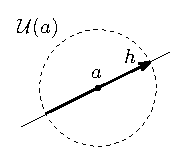
\includegraphics[width=0.15\textwidth]{18_2.eps}
		\caption{$a$ - локальный экстремум на прямой внутри окрестности $\MU(a)$.}
		\label{18_2}
	\end{figure}
	Следовательно, для одномерных функций мы знаем, что из этого следует $\varphi^\prime(0) = 0 \Rightarrow df(a,h) = 0$
\end{proof}
\begin{theorem}\textbf{(достаточное условие локального экстремума)}
	Пусть $f$ дважды дифференцируема в окрестности точки $a$ и её вторые производные непрерывны в точке $a$. Предположим, что $df(a,h) = 0, \, \forall h$. Тогда будет верно следующее:
	\begin{enumerate}[label ={(\arabic*)}]
		\item Если $d^2f(a,h) > 0, \, \forall h \neq 0$, то $a$ - точка строгого локального минимума;
		\item Если $d^2f(a,h) < 0, \, \forall h \neq 0$, то $a$ - точка строгого локального максимума;
		\item Если $\exists \, h,v \colon d^2f(a,v) < 0 \wedge d^2f(a,h) > 0$, то $a$ не является точкой локального экстремума; 
	\end{enumerate}
\end{theorem}
\begin{rem}
	Непрерывность вторых производных - избыточное требование.
\end{rem}
\begin{rem}
	Подход сведения ситуации к прямым не верен при исследовании экстремумов (провести через точку $a$ прямую и на этой прямой - одномерная функция, для неё мы знаем как определять тип экстремума). Далее, мы посмотрим пример почему это не так: есть строгий экстремум по каждой прямой, но при этом нет экстремума по совокупности переменных в этой точке.
\end{rem}
\textbf{Пример}: Рассмотрим функцию $f(x,y) = x^4 + y^2$, очевидно что $(0,0)$ - точка строгого локального минимума, второй дифференциал: 
$$
	d^2f(0,0) = 2(dy)^2
$$
Он не относится ни к одному из случаев, поскольку подставляя $h$ в дифференциал получим: $$
	d^2f(h) = 2h_2^2
$$ 
Следовательно нельзя утверждать, что на всех векторах это положительное значение (например, если вторая координата равна нулю: $h_2 = 0 \Rightarrow d^2f(h) = 0$), нет двух разнознаковых направлений $\Rightarrow$ не подпадает ни под один из случаев и второй дифференциал даже не занулился, то есть он просто выродился. При этом есть точка строгого локального минимума.

\textbf{Пример}: Рассмотрим функцию $f(x,y) = x^3 + y^2$, точка $(0,0)$ теперь перестала быть точкой строгого локального минимума, но при этом $d^2f = 2(dy)^2$.
\begin{proof}\hfill
	\begin{enumerate}[label ={(\arabic*)}]
		\item По условию $d^2f(a,h) > 0, \, \forall h \neq 0$. Разложим исходную функцию по формуле Тейлора:
		$$
			f(a + h) = f(a) + df(a,h) +  \dfrac{d^2f(a,h)}{2} + \overline{o}(\|h\|^2) = f(a) + 0 +  \dfrac{d^2f(a,h)}{2} + \overline{o}(\|h\|^2)
		$$
		Распишем подробнее остаточный член. Поскольку $d^2f(a,h)$ - квадратичное выражение, то вынесем за скобки $\|h\|^2$ и получим:
		$$
			\dfrac{d^2f(a,h)}{2} + \overline{o}(\|h\|^2) =\|h\|^2{\cdot}\bigg(\dfrac{1}{2}{\cdot}d^2f\bigg(a,\dfrac{h}{\|h\|}\bigg) + \overline{o}(1) \bigg), \, \dfrac{h}{\|h\|} \in \{v \colon \|v\| = 1\}
		$$
		Рассмотрим следующее отображение: $v \mapsto d^2(a,v)$, оно непрерывно как квадратичная форма. Отметим также, что $\{v \colon \|v\| = 1\}$ это компакт (ограниченное и замкнутое). Тогда на этом компакте непрерывная функция достигает своего минимума. Пусть: 
		$$
			m = \min\limits_{\|v\| = 1}d^2f(a,v) \Rightarrow \forall h \neq 0, \, d^2f\bigg(a,\dfrac{h}{\|h\|}\bigg) \geq m
		$$
		Поскольку он достигается по теореме Вейрштрасса и $d^2f(a,h) > 0, \, \forall h \neq 0$ по условию, то $m > 0$. Тогда, при достаточно малых $h$, получим:
		$$
			f(a + h) - f(a) \geq \|h\|^2{\cdot}\bigg(\dfrac{m}{2} + \overline{o}(1)\bigg) > 0, \, \lim\limits_{h \to 0} \overline{o}(1) = 0
		$$
		\item По условию $d^2f(a,h) < 0, \, \forall h \neq 0$. Аналогично первому пункту, на компакте непрерывная функция достигнет своего максимума. Пусть:
		$$
			M = \max\limits_{\|v\| = 1}d^2f(a,v) \Rightarrow \forall h \neq 0, \, d^2f\bigg(a,\dfrac{h}{\|h\|}\bigg) \leq M
		$$
		Поскольку он достигается по теореме Вейрштрасса и $d^2f(a,h) < 0, \, \forall h \neq 0$ по условию, то $M < 0$. Тогда, при достаточно малых $h$, получим:
		$$
			f(a + h) - f(a) \leq \|h\|^2{\cdot}\bigg(\dfrac{M}{2} + \overline{o}(1)\bigg) < 0, \, \lim\limits_{h \to 0} \overline{o}(1) = 0
		$$
		\item Пусть $\exists \, h, \, v \colon d^2f(a,v) < 0 , \, d^2f(a,h) > 0$. Рассмотрим функции $\varphi_1(t) = f(a + tv)$ и $\varphi_2(t) = f(a + th)$:
		\begin{figure}[H]
			\centering
			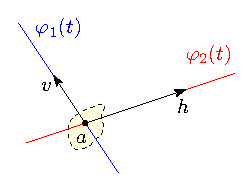
\includegraphics[width=0.25\textwidth]{18_3.eps}
			\caption{Функции $\varphi_1(t)$ и $\varphi_2(t)$ по направлениям $v$ и $h$.}
			\label{18_3}
		\end{figure}
		Мы знаем, что для $\varphi_1(t)$:
		$$
			\varphi_1^\prime(0) = df(a,v) = 0, \, \varphi_1^{\prime\prime}(0) = d^2f(a,v) < 0
		$$ 
		Следовательно, точка $0$ для $\varphi_1(t)$ это точка строгого локального максимума. Аналогично для $\varphi_2(t)$: 
		$$
			\varphi_2^\prime(0) = df(a,h) = 0, \, \varphi_2^{\prime\prime}(0) = d^2f(a,h) > 0
		$$ 
		Следовательно, точка $0$ для $\varphi_2(t)$ это точка строгого локального минимума. Таким образом, в окрестности точки $a$ мы найдем как точки в которых значения строго меньше, чем значение в точке $a$, так и точки в которых значения строго больше, чем значение в точке $a$. Значит эта точка не является точкой экстремума.
	\end{enumerate}
\end{proof}

Как уже упомянали, ограничение на прямую в функциях многих переменных для поиска экстремумов является не верным подходом. Рассмотрим иллюстрирующий пример.

\textbf{Пример}: Обозначим через $h(x,y)$ знакомую нам функцию: $h(x,y) = 
	\begin{cases} 
		-1, & y = x^2 \wedge x \geq 0 \\ 
		0, & y \neq x^2 \vee x < 0 
	\end{cases}
$. И рассмотрим функцию $f(x,y) = x^2 + y^2 + h(x,y)$. Посмотрим, что у этой функции в точке $(0,0)$.
\begin{figure}[H]
	\centering
	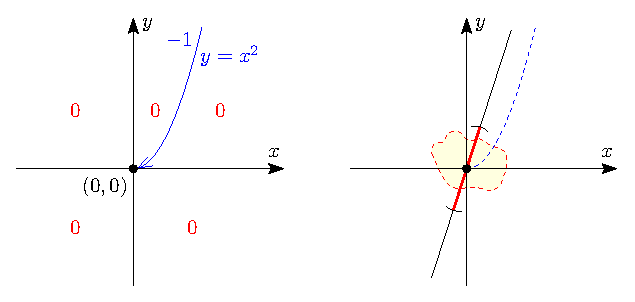
\includegraphics[width=0.6\textwidth]{18_4.eps}
	\caption{Функции $h(x,y)$ и окрестность точки $(0,0)$ функции $f(x,y)$.}
	\label{18_4}
\end{figure}
Какую бы проходящую через ноль прямую мы не взяли, найдется окрестность, где $h(x,y) = 0 \Rightarrow$ на этой окрестности $f(x,y) = x^2 + y^2$, которая в $(0,0)$ будет иметь строгий локальный минимум. Но по совокупности двух переменных это не так: если мы возьмем точки вдоль $y = x^2$, то точки $x^2 + y^2$ будут стремиться к нулю, а $h(x,y) = -1 \Rightarrow$ сколь угодно близко к нулю есть точки, где $f(x,y) < 0$. 

Таким образом в любой окрестности нуля есть как точки с $f(x,y) > 0$, так и точки с $f(x,y) < 0$. У функции $f(x,y)$ по каждой прямой в $(0,0)$ - строгий локальный минимум, но при этом настоящего локального минимума по совокупности переменных нет.
\begin{rem}
	В качестве $h(x,y)$ можно взять сглаженную функцию и тогда получим гладкую функцию для которой данное наблюдение останется верным.
\end{rem}

\section*{Условный экстремум}
\textbf{\uline{Задача (летний кинотеатр)}}: На высоте $h$ от уровня обзора висит экран шириной $H$. Где лучше сесть вдоль линии обзора, чтобы был максимальным угол $\varphi$ под которым видим этот экран?
\begin{figure}[H]
	\centering
	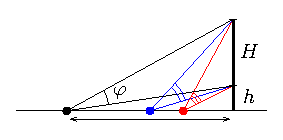
\includegraphics[width=0.3\textwidth]{18_5.eps}
	\caption{Задача про летний кинотеатр: поиск места с лучшим углом обзора $\varphi$.}
	\label{18_5}
\end{figure}
Перед нами стоит задача $\varphi \to \max$. Поймем для начала, откуда угол обзора будет одинаковым. Из школы известно, что вписанные углы, опирающиеся на одну и ту же хорду равны.
\begin{figure}[H]
	\centering
	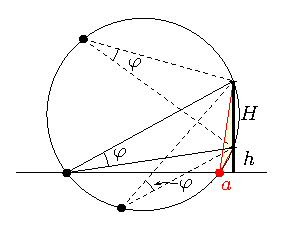
\includegraphics[width=0.3\textwidth]{18_6.eps}
	\caption{Вписанные углы, опирающиеся на одну и ту же хорду равны.}
	\label{18_6}
\end{figure}
В частности, угол в точке $a$ на рисунке также будет равен $\varphi$. Но из точек на линии обзора (т.е. которые опираются на ту же дугу внутри круга) углы будет больше. 

Хотим понять, в каком случае невозможно будет увеличить угол под которым видим экран? Только тогда, когда не будет точек внутри круга на линии обзора $\Rightarrow$ нужно взять окружность, которая будет опираться на хорду экрана и касаться линии обзора.
\begin{figure}[H]
	\centering
	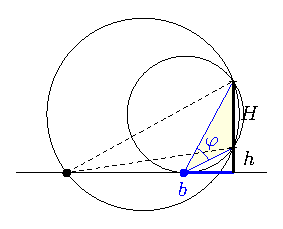
\includegraphics[width=0.3\textwidth]{18_7.eps}
	\caption{Максимальный угол обзора в точке $b$.}
	\label{18_7}
\end{figure}
Расстояние до искомой точки $b$ от экрана по теореме о секущей и касательной будет равно $\sqrt{(h+H)h}$.

Что мы делали, когда начали смотреть на эти окружности? 
\begin{figure}[H]
	\centering
	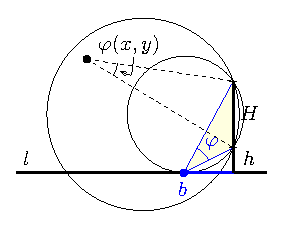
\includegraphics[width=0.3\textwidth]{18_8.eps}
	\caption{Задача на условный экстремум.}
	\label{18_8}
\end{figure}
Была функция $\varphi(x,y)$ которая в точке $(x,y)$ сообщает нам угол под которым мы видим экран. Мы искали экстремум (максимум) этой функции, при условии что точки $(x,y)$ лежат на некотором множестве (в данном случае это прямая) $l$:
$$
\left\{
	\begin{array}{l}
		\varphi(x,y) \to \text{extr}!\\
		(x,y) \in l
	\end{array}
\right.
$$
То есть, мы получили стандартную задачу на условный экстремум: ищем экстремум функции, но при этом разрешается брать не любые точки, а удовлетворяющие некоему условию. Чтобы решить эту задачу мы начали рисовать множества уровняей функции: $\varphi(x,y) = \varphi_0$. И мы нашли решение в точке, где линия уровня $\varphi$ коснулась линии, которая задает нам условие.

\textbf{\uline{Идея}}: Ищем экстремумы в тех точках, в которых линии уровня исследуемой функции касаются линии задающей условия.

\textbf{\uline{Задача}}: Еще одной типичной задачей на условный экстремум является поиск экстремума на единичной окружности:
$$
\left\{
\begin{array}{l}
	x + y \to \text{extr}!\\
	x^2 + y^2  = 1
\end{array}
\right.
$$
В этом случае рисуем окружность, проводим линии уровня и исследуем точки соприкосновения.
\end{document}